
\begin{figure}
\begin{center}
\begin{tabular}{cc}
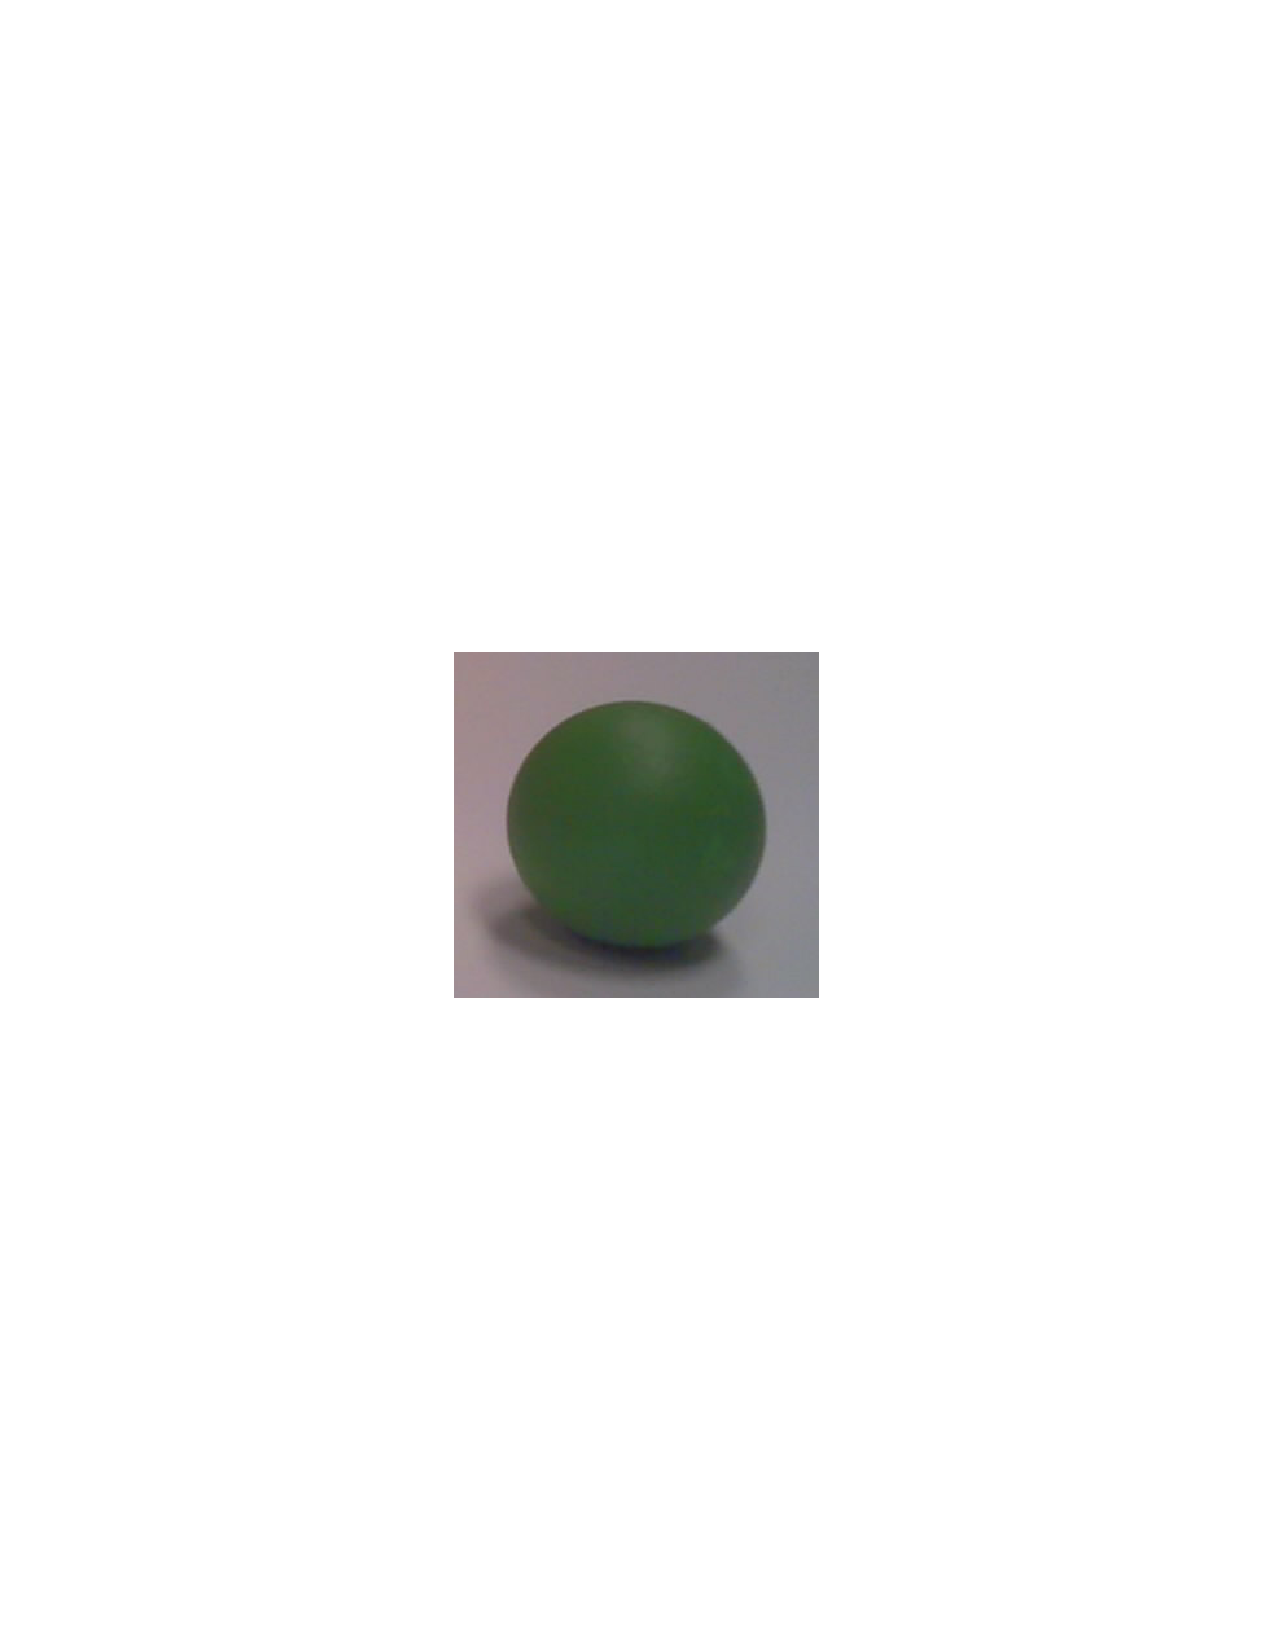
\includegraphics[trim=190 280 190 290,clip,width=0.48\linewidth]{Figures/sphereColor} &
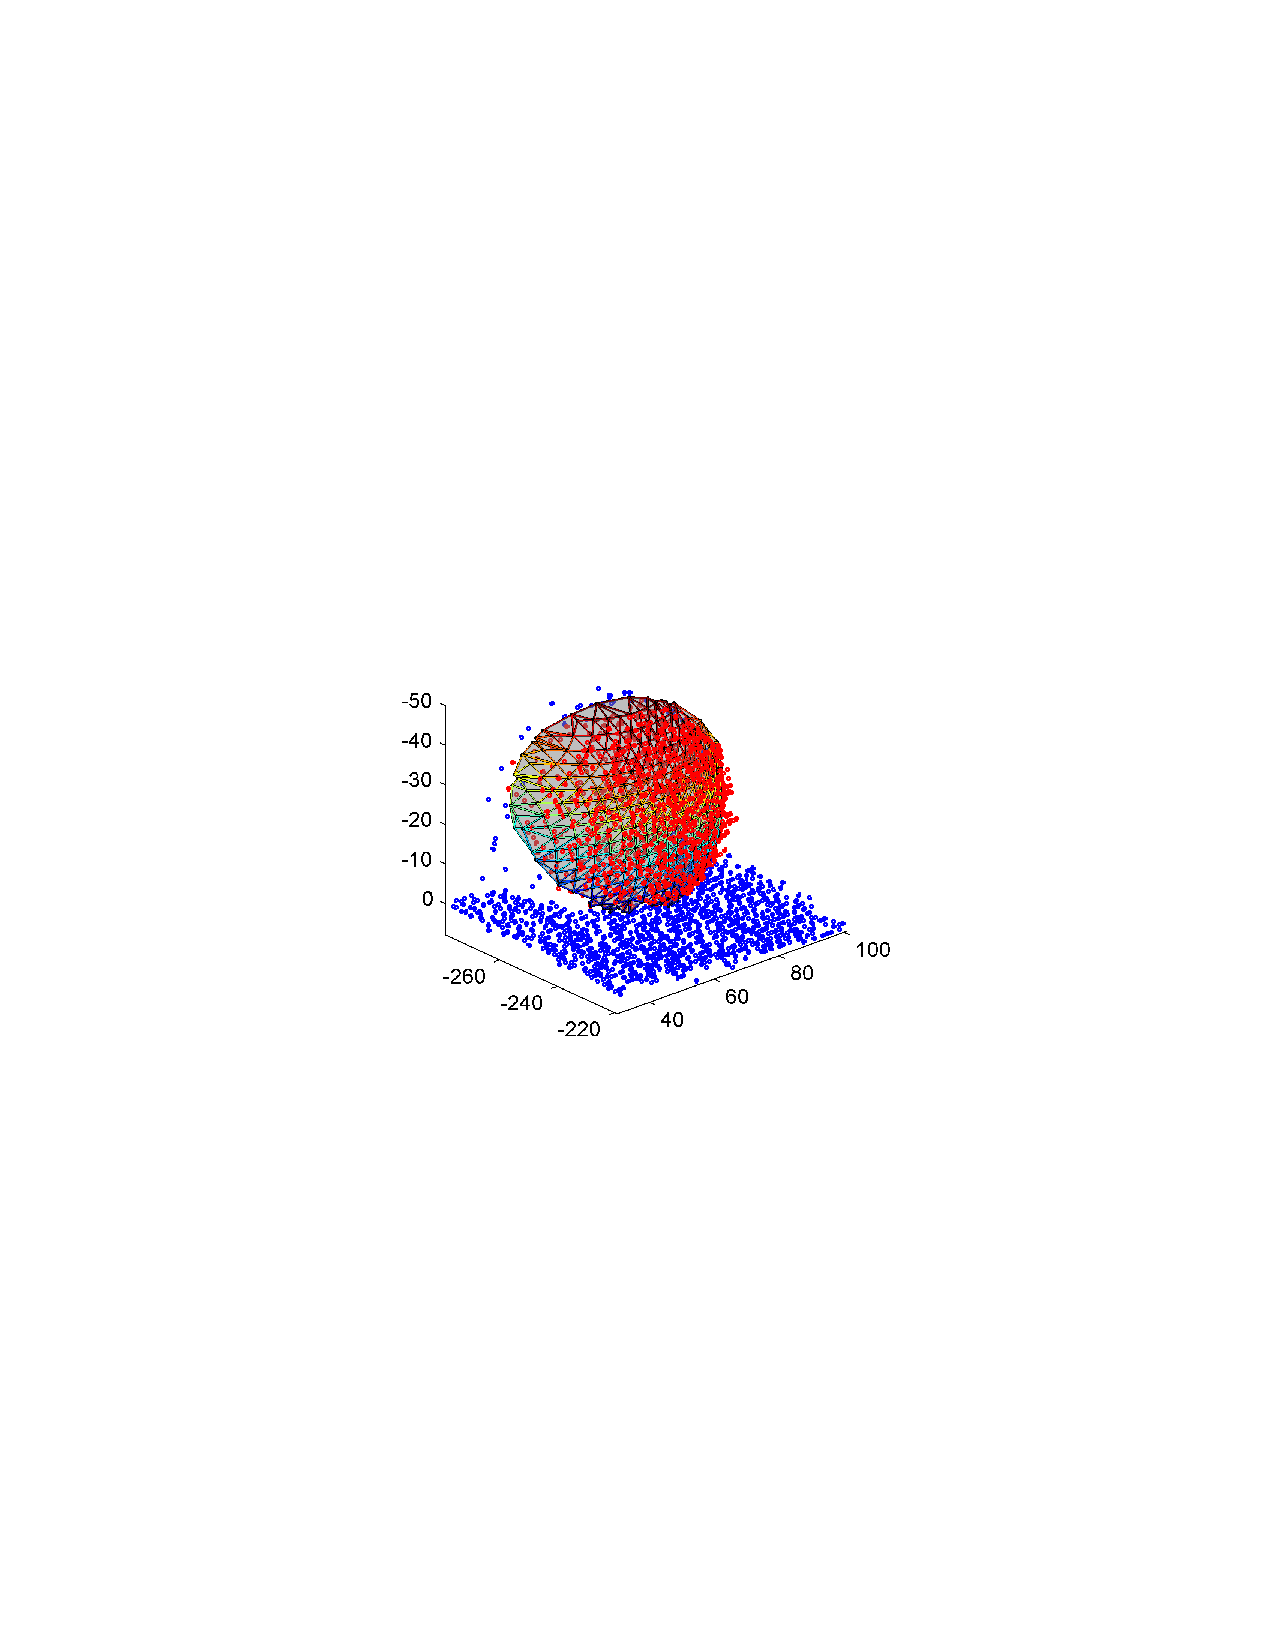
\includegraphics[trim=190 280 190 290,clip,width=0.48\linewidth]{Figures/sphere3DMesh} \\
($a$) & ($b$) \\
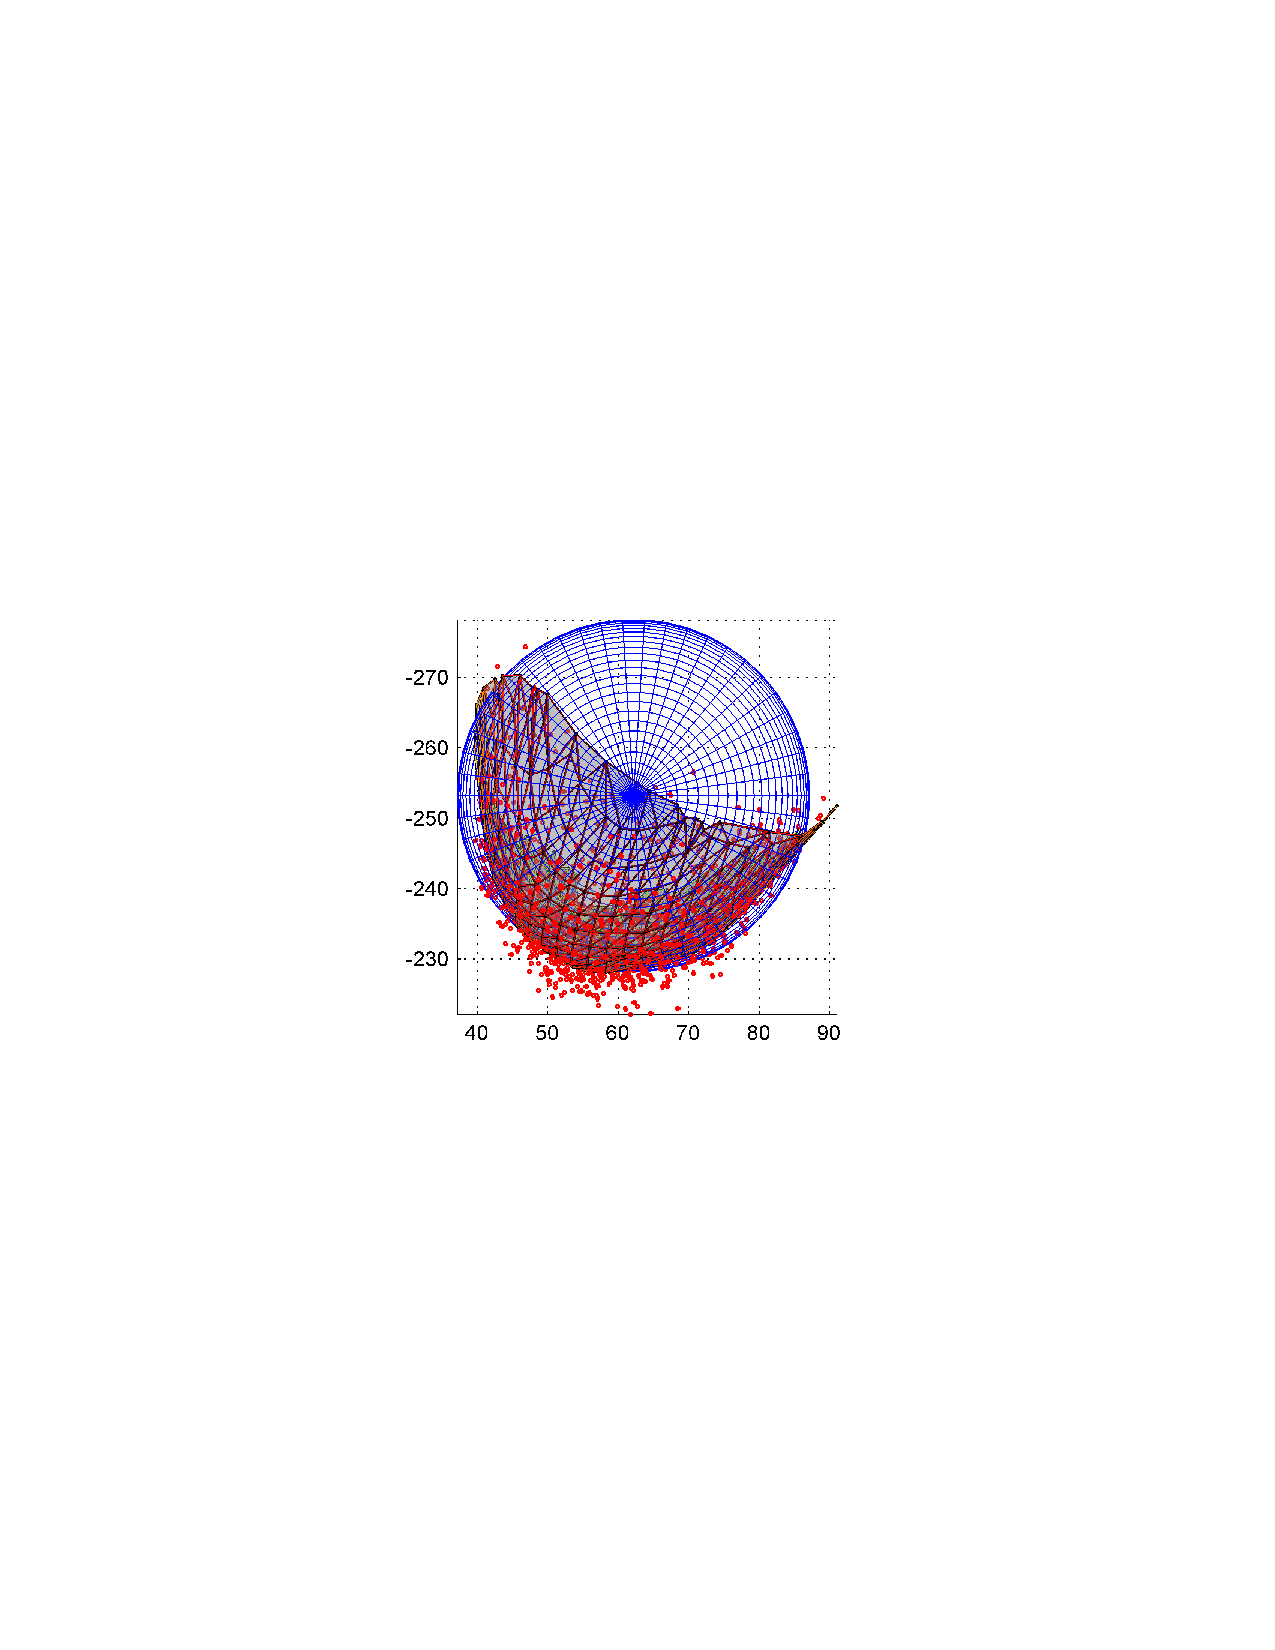
\includegraphics[trim=190 280 190 290,clip,width=0.48\linewidth]{Figures/sphere3DMeshWithGT} &
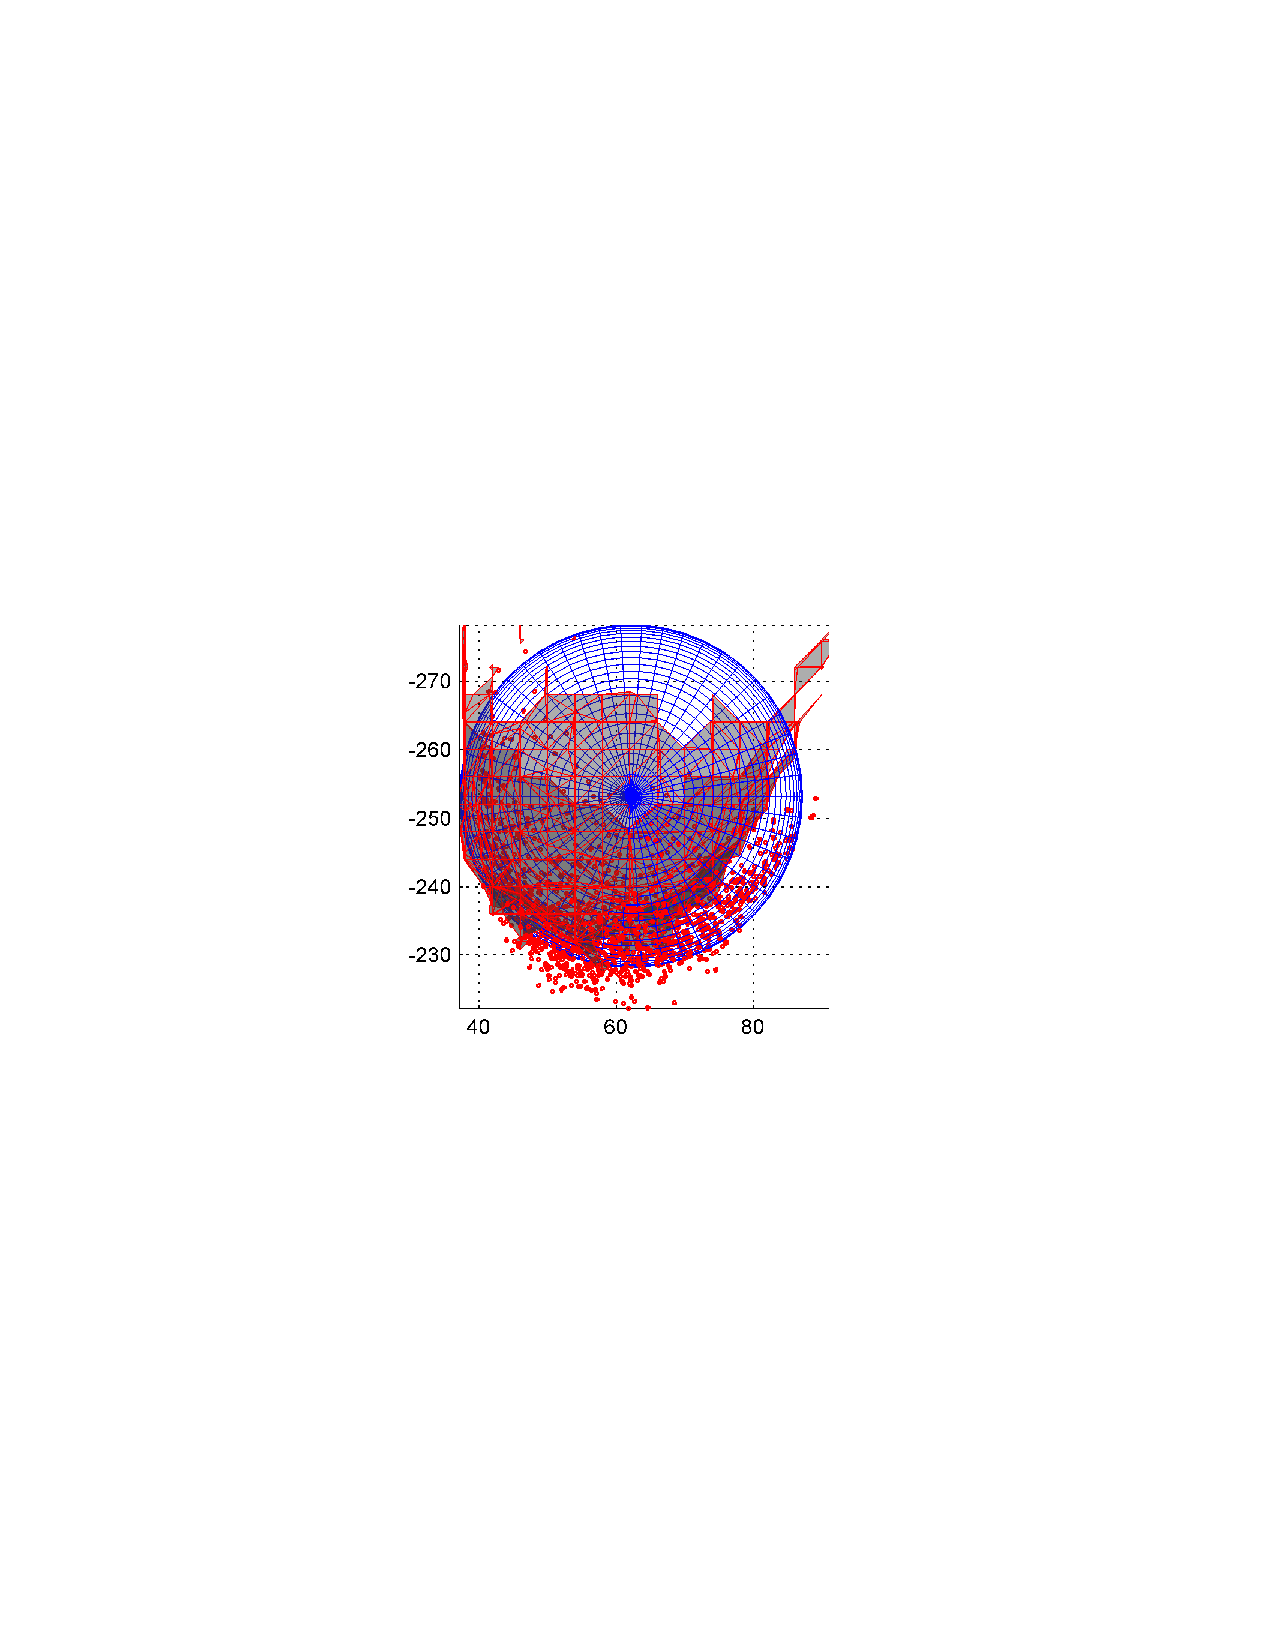
\includegraphics[trim=190 280 190 290,clip,width=0.48\linewidth]{Figures/sphere3DIsosurface} \\
($c$) & ($d$) \\
\end{tabular}
\end{center}
   \caption{($a$) Color image of a 50mm diameter sphere.  ($b$) Estimated $3$D mesh. ($c$) Known sphere shape with center fit to data points shows how well the mesh captures the real surface.  ($d$) The isosurface is much more jagged and does not fit as well.  }
\label{fig:sphere}
\end{figure}


\begin{figure}
\begin{center}
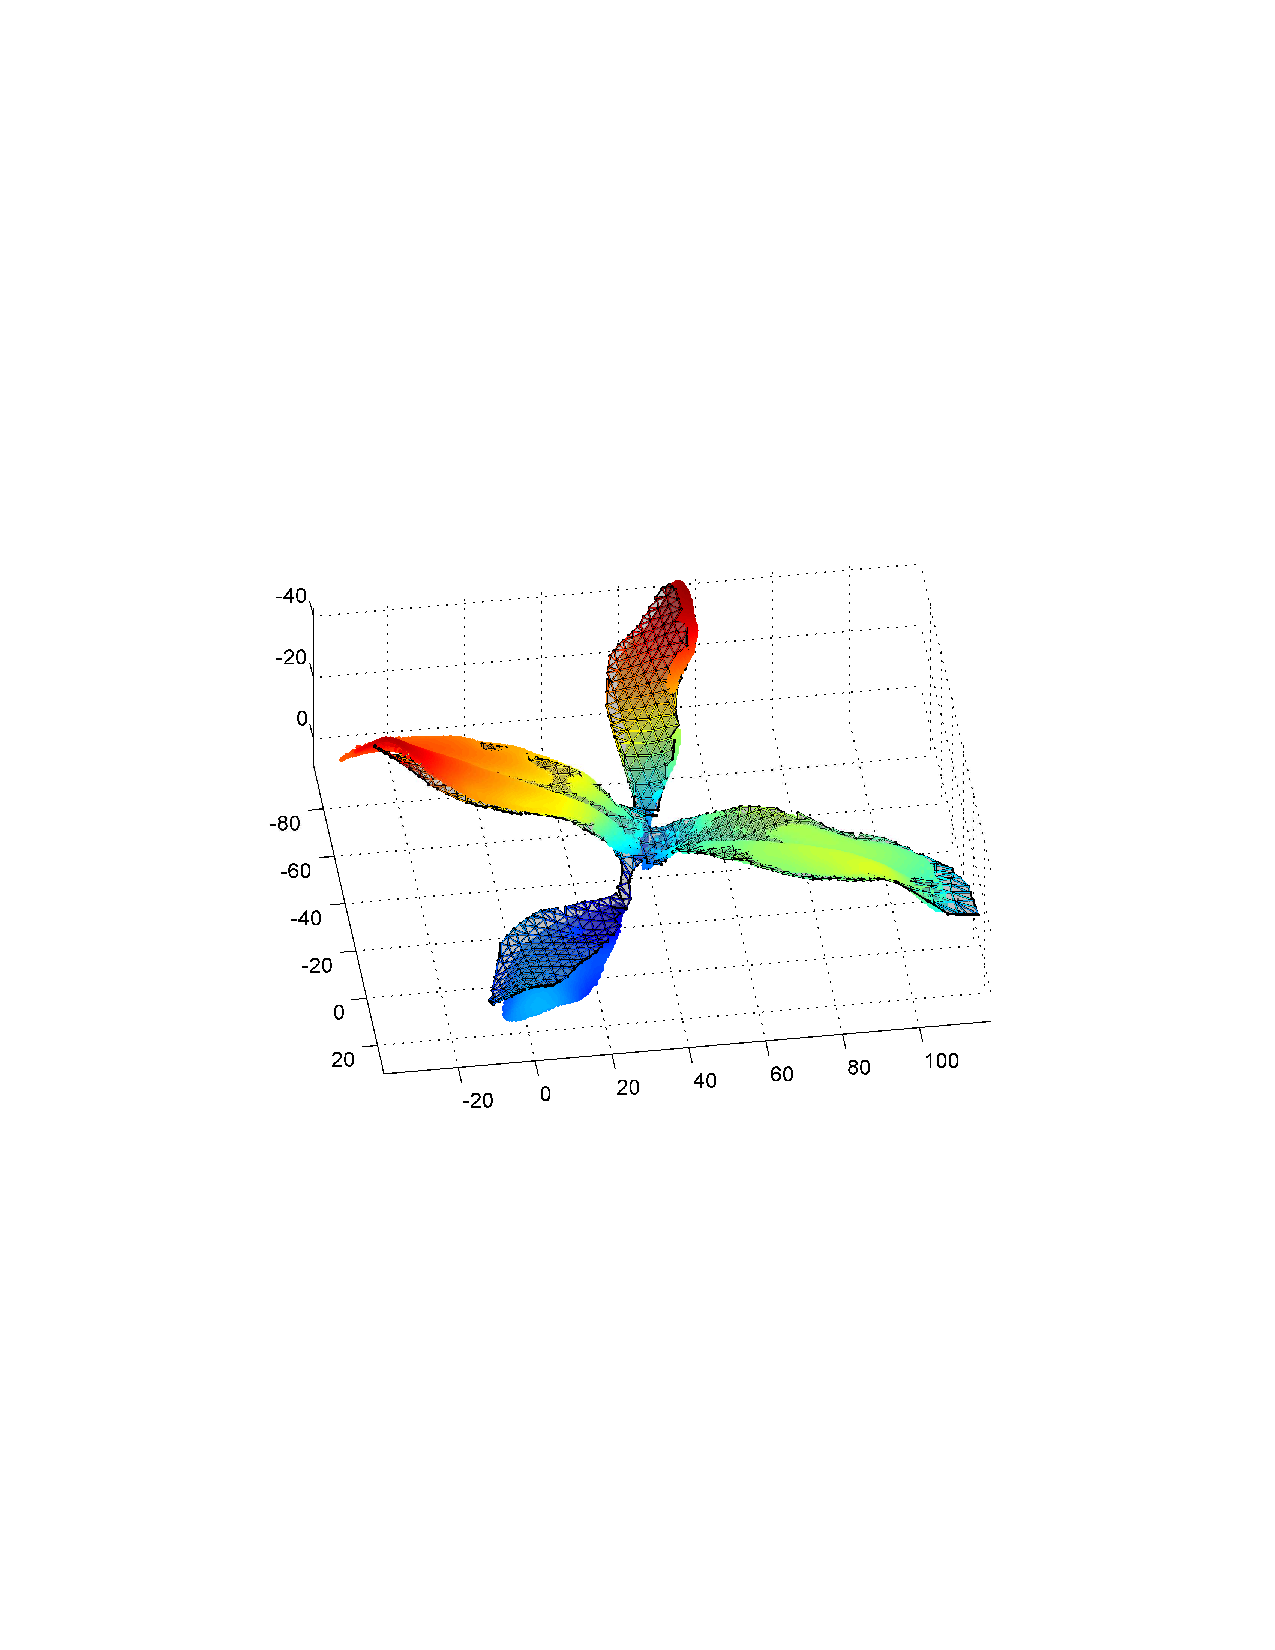
\includegraphics[trim=120 220 120 220,clip,width=0.7\linewidth]{Figures/plantMeshGT-01}
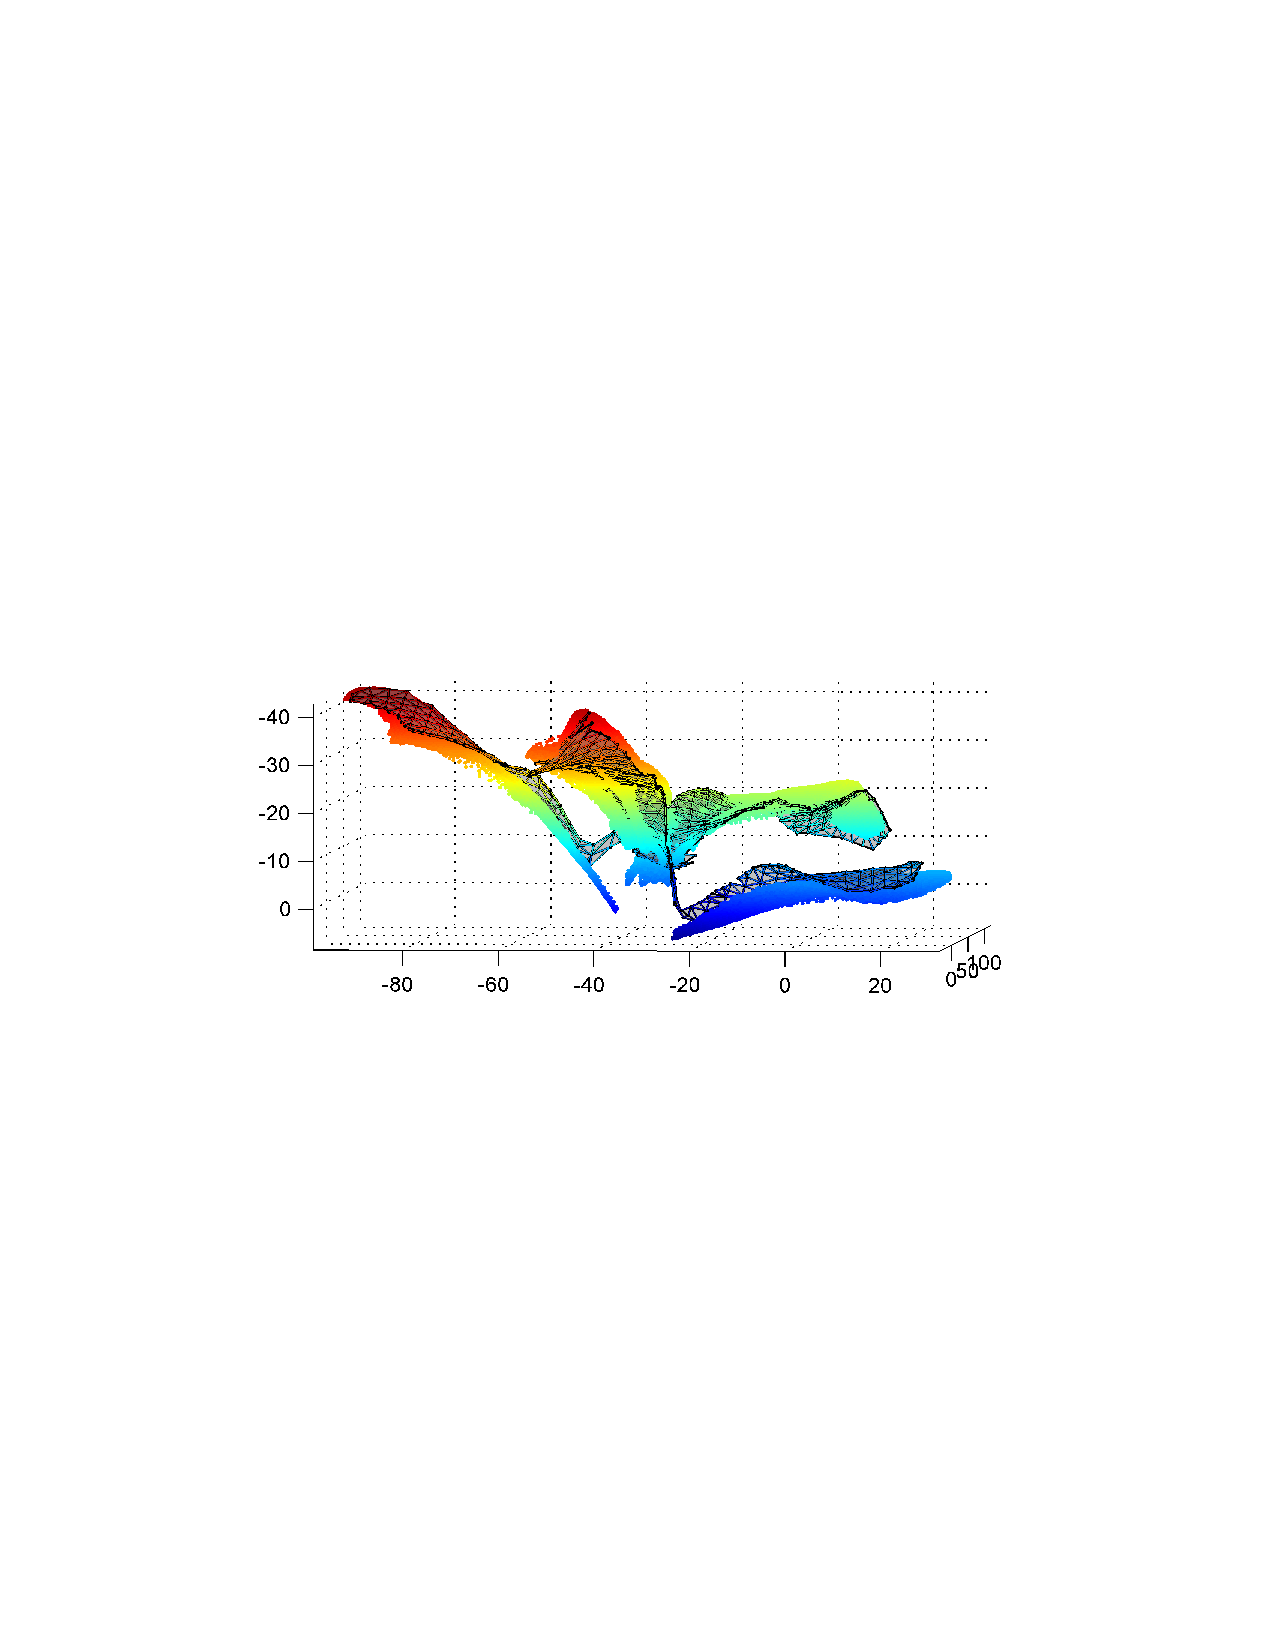
\includegraphics[trim=120 300 120 300,clip,width=0.7\linewidth]{Figures/plantMeshGT-02}
\end{center}
   \caption{ The $3$D reconstruction from Fig.~\ref{fig:plantnoise} is aligned to a laser scan of the plant image. The laser scan data are shown as smoothly-colored surfaces plotted in the same axes as the mesh.  The two views show good overall agreement including feature curves. Errors are seen near the ends of the left and right leaves.  The lower leaf has likely shifted between the laser scan and the depth data collection.  }
\label{fig:plantnoiseGT}
\end{figure}

\begin{figure}
\begin{center}
\begin{tabular}{c}
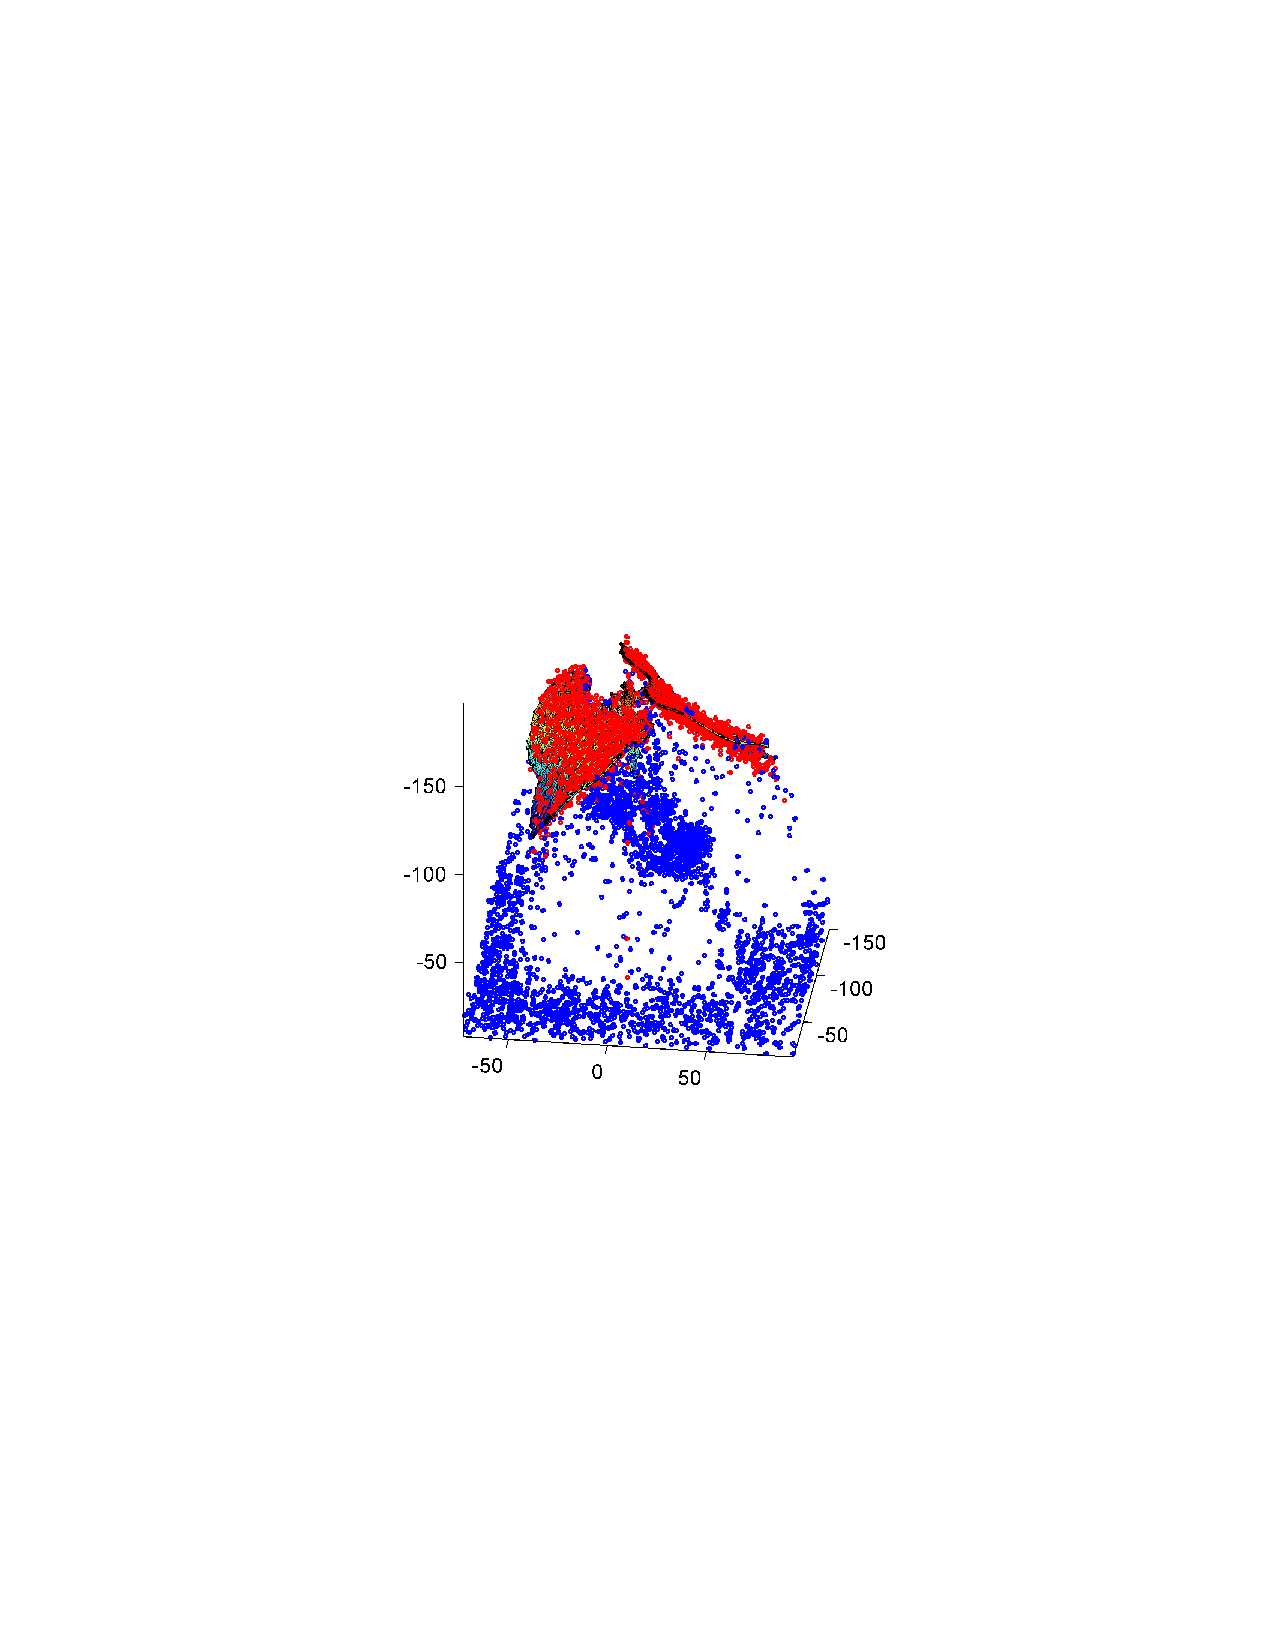
\includegraphics[trim=190 270 190 290,clip,width=0.7\linewidth]{Figures/bean3DMeshPlusPoints} \\
($a$) \\
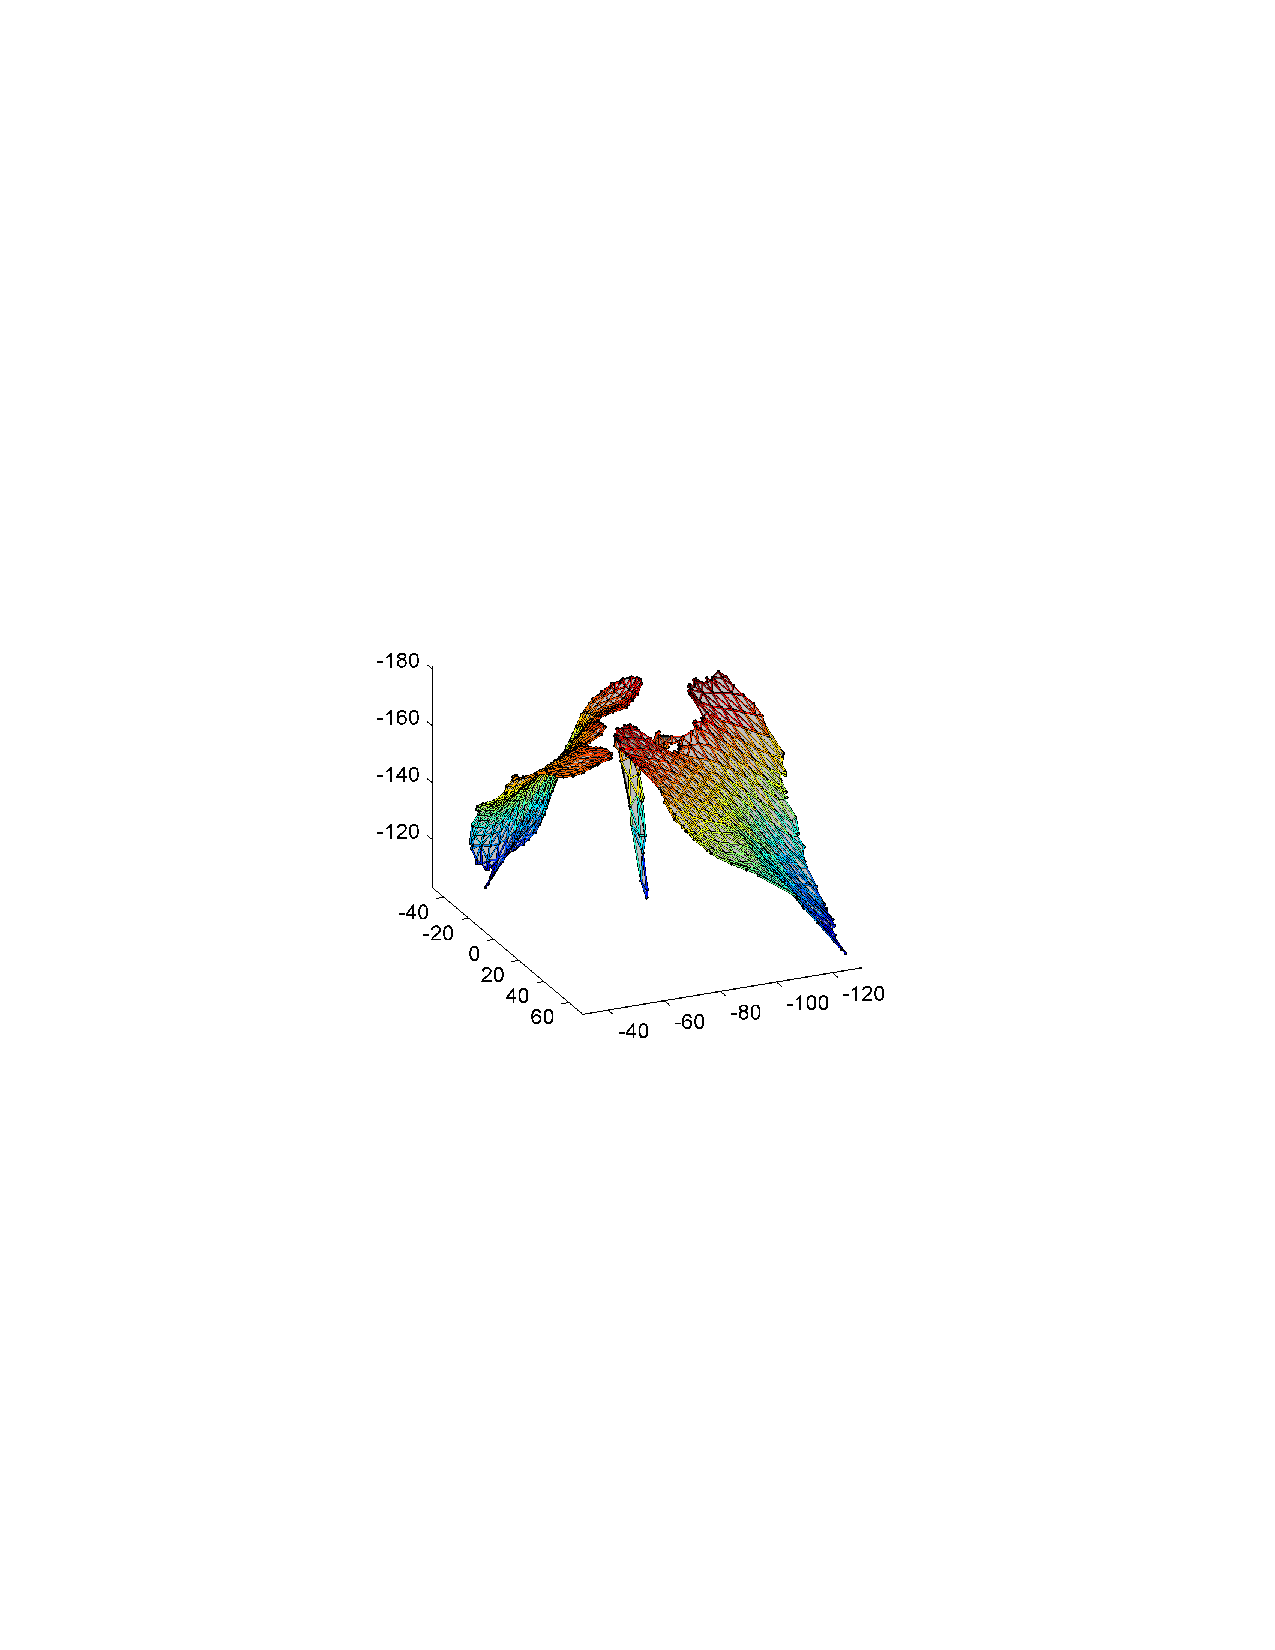
\includegraphics[trim=190 280 190 290,clip,width=0.7\linewidth]{Figures/bean3DMesh} \\
($b$) \\
\end{tabular}
\begin{tabular}{cc}
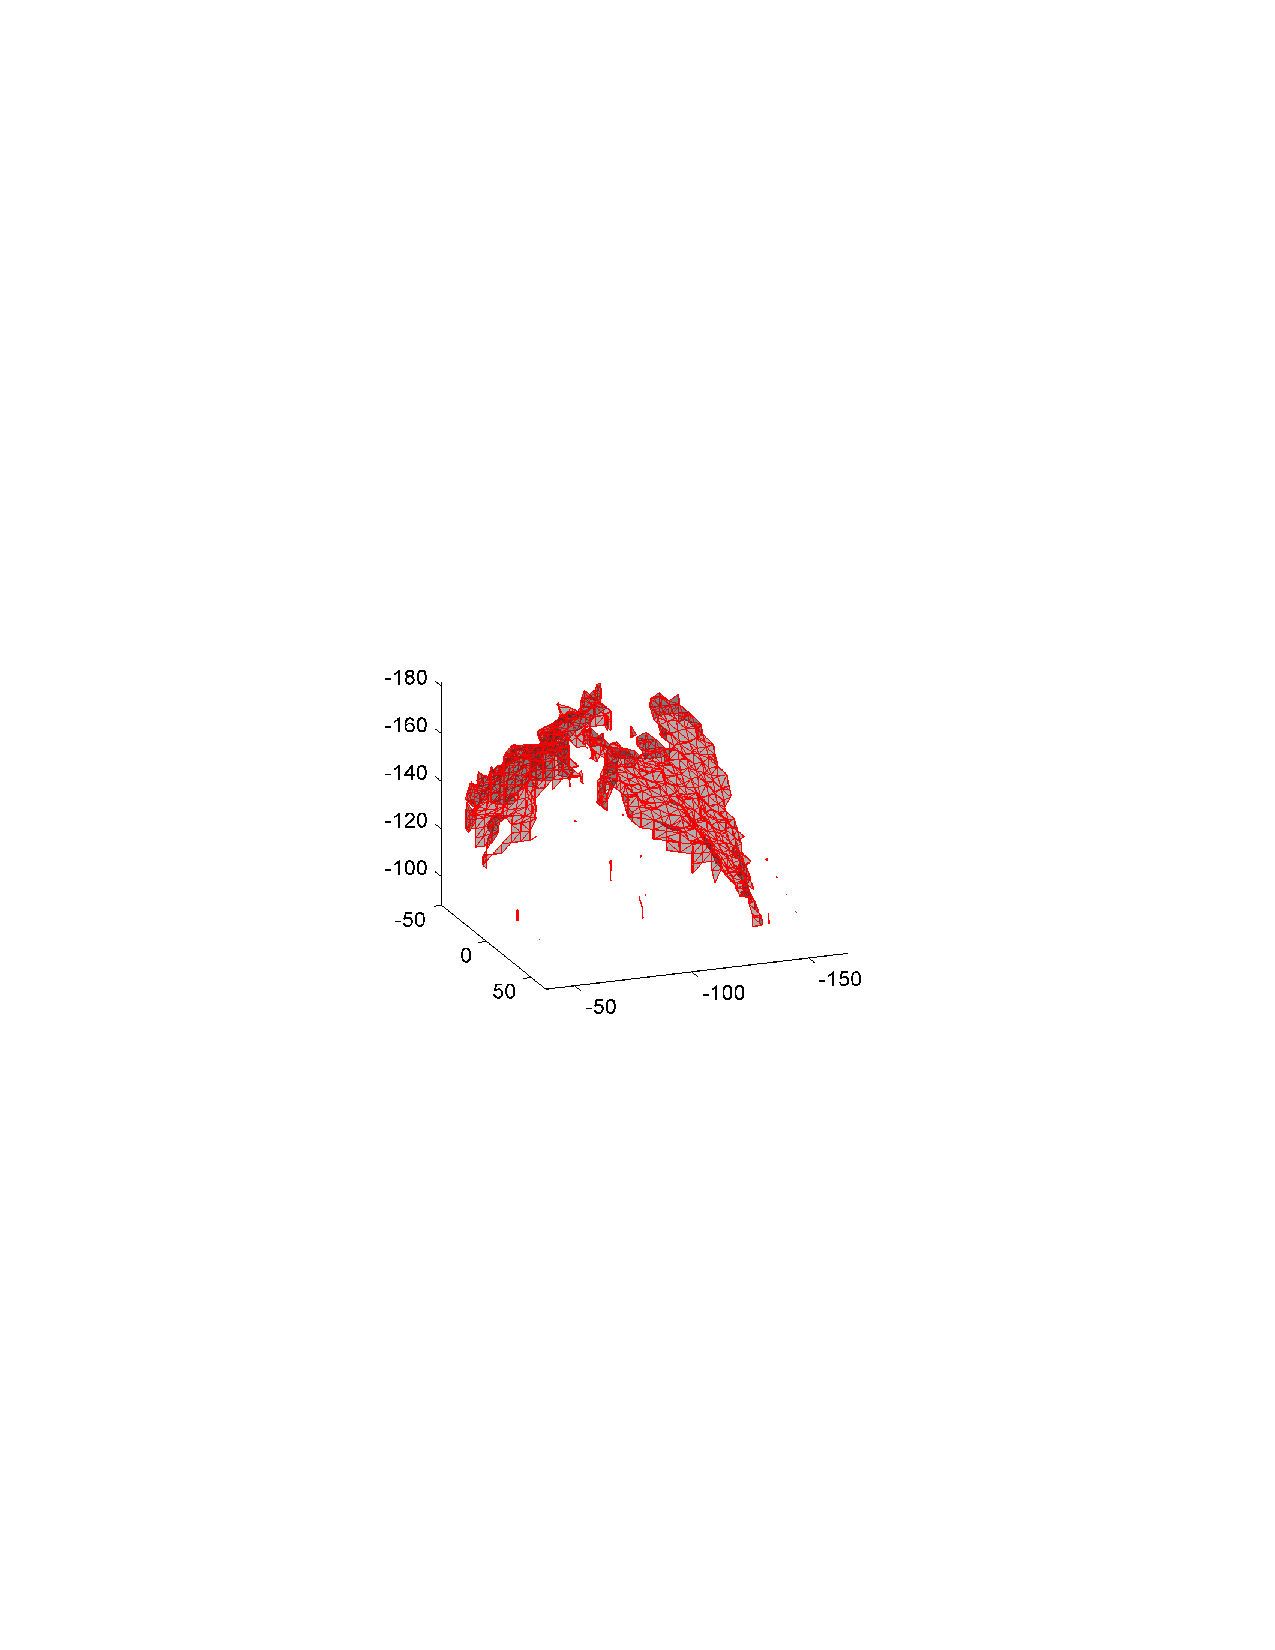
\includegraphics[trim=190 280 190 290,clip,width=0.49\linewidth]{Figures/bean3DIsosurface} &
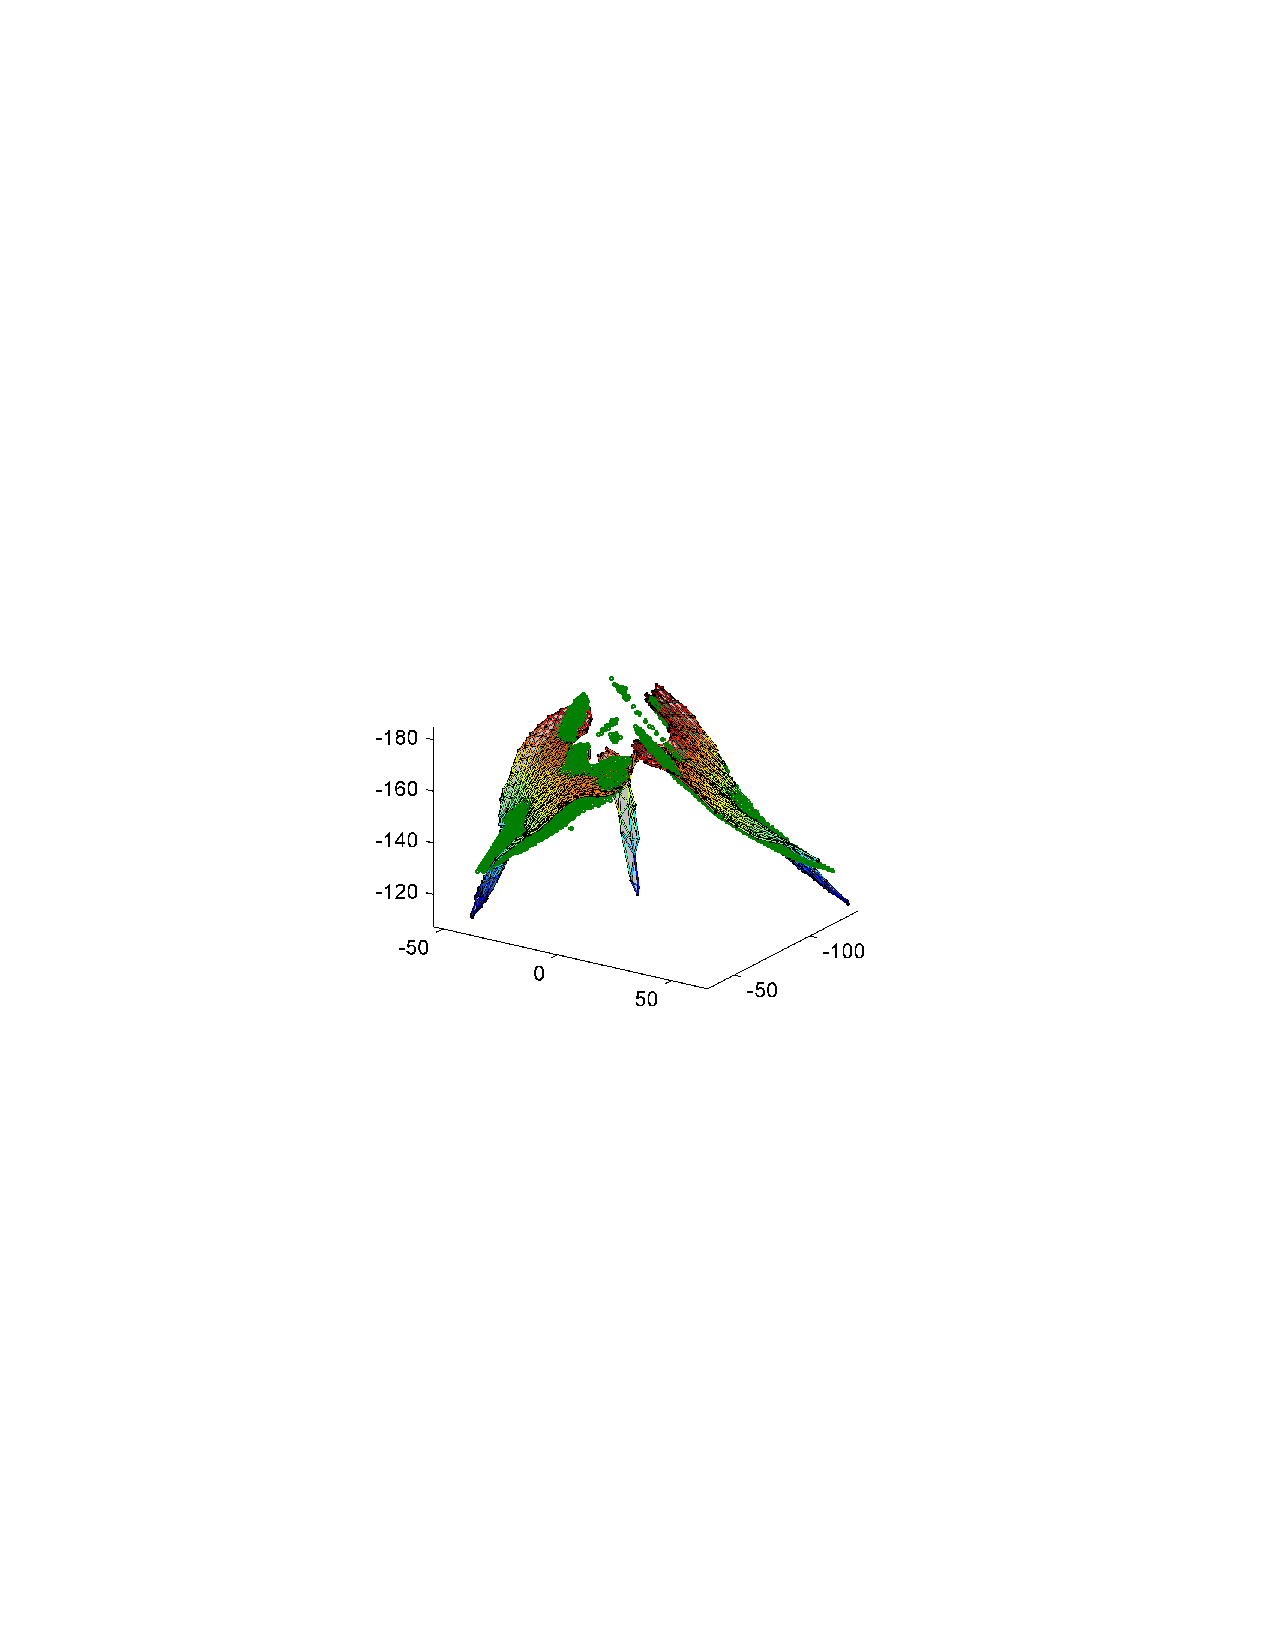
\includegraphics[trim=190 280 190 290,clip,width=0.49\linewidth]{Figures/beanParabolic} \\
($c$) & ($d$) \\
\end{tabular}
\end{center}
   \caption{ Result of fitting the mesh to the bean data from Fig.~\ref{fig:beanimageprocess}.  ($a$)  The $3$D points are red for those on the mesh and blue for the remaining.  ($b$) A more detailed view of the mesh revealing detailed curves of the leaves. ($c$) A comparison with an isosurface created using marching cubes~\cite{Curless:1996}. ($d$) A comparison with the use of parabolic fits to leaf surfaces (dark green points) as used in~\cite{Alenya2011,Alenya2013}.  Clearly parabolic models cannot capture complex bean leaf structures or the leaves in Fig.~\ref{fig:plantnoiseGT}. }
\label{fig:beanfit}
\end{figure}

\begin{figure}
\begin{center}
\begin{tabular}{cc}
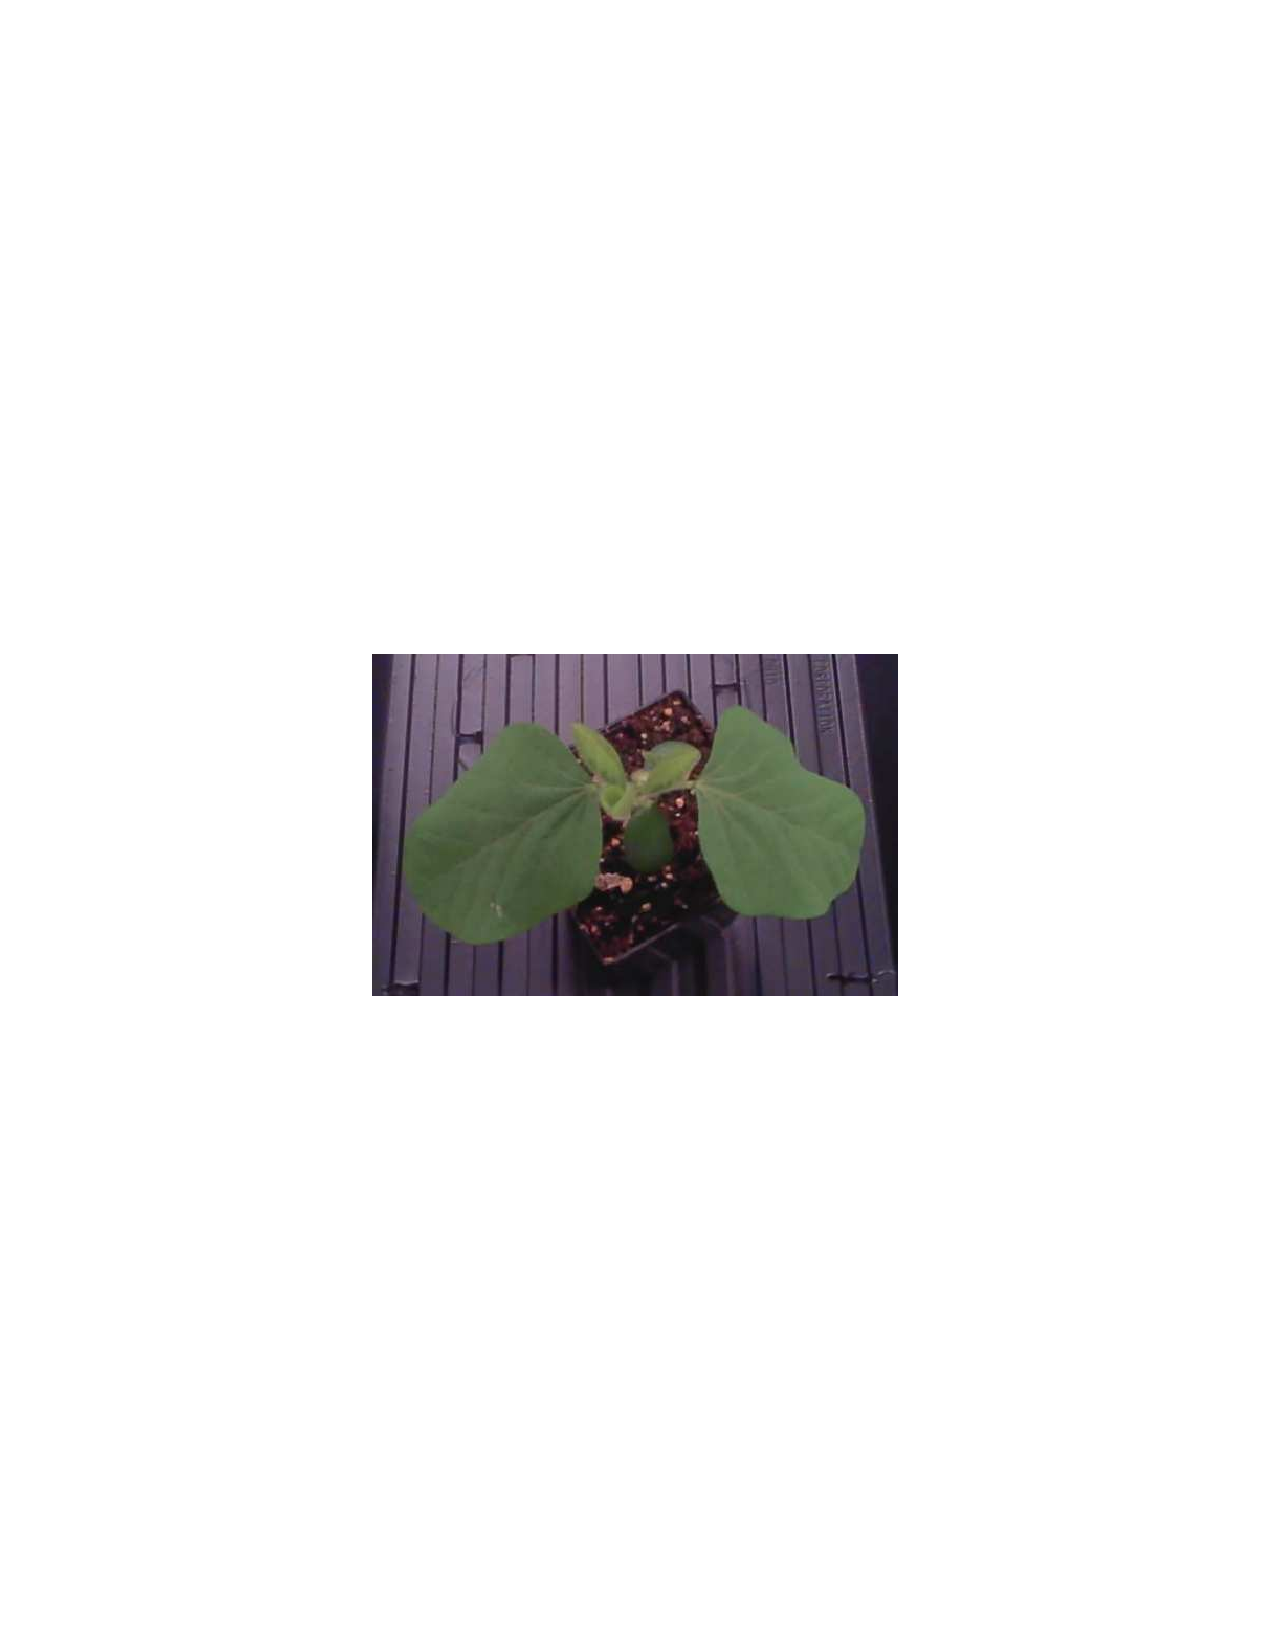
\includegraphics[trim=190 280 190 290,clip,width=0.48\linewidth]{Figures/soybeanColor} &
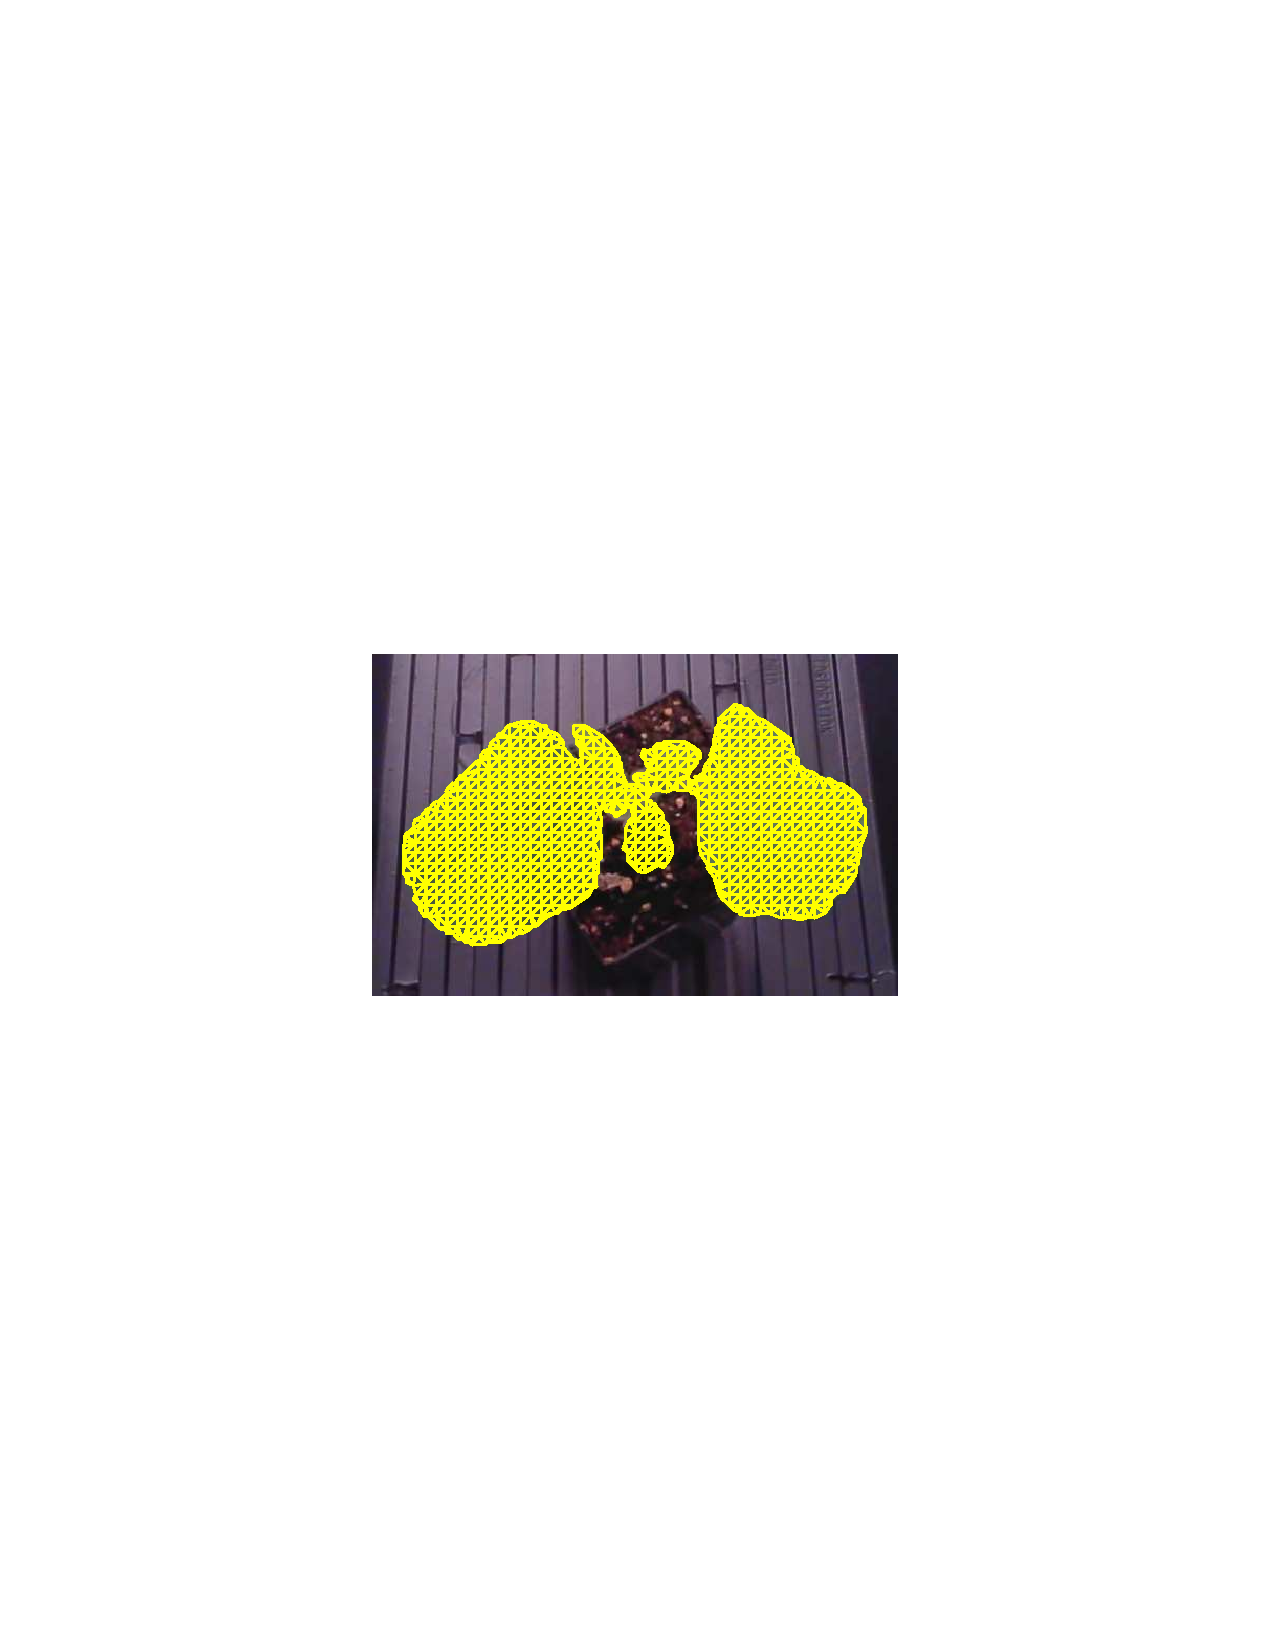
\includegraphics[trim=190 280 190 290,clip,width=0.48\linewidth]{Figures/soybeanColorMesh} \\
($a$) & ($b$) \\
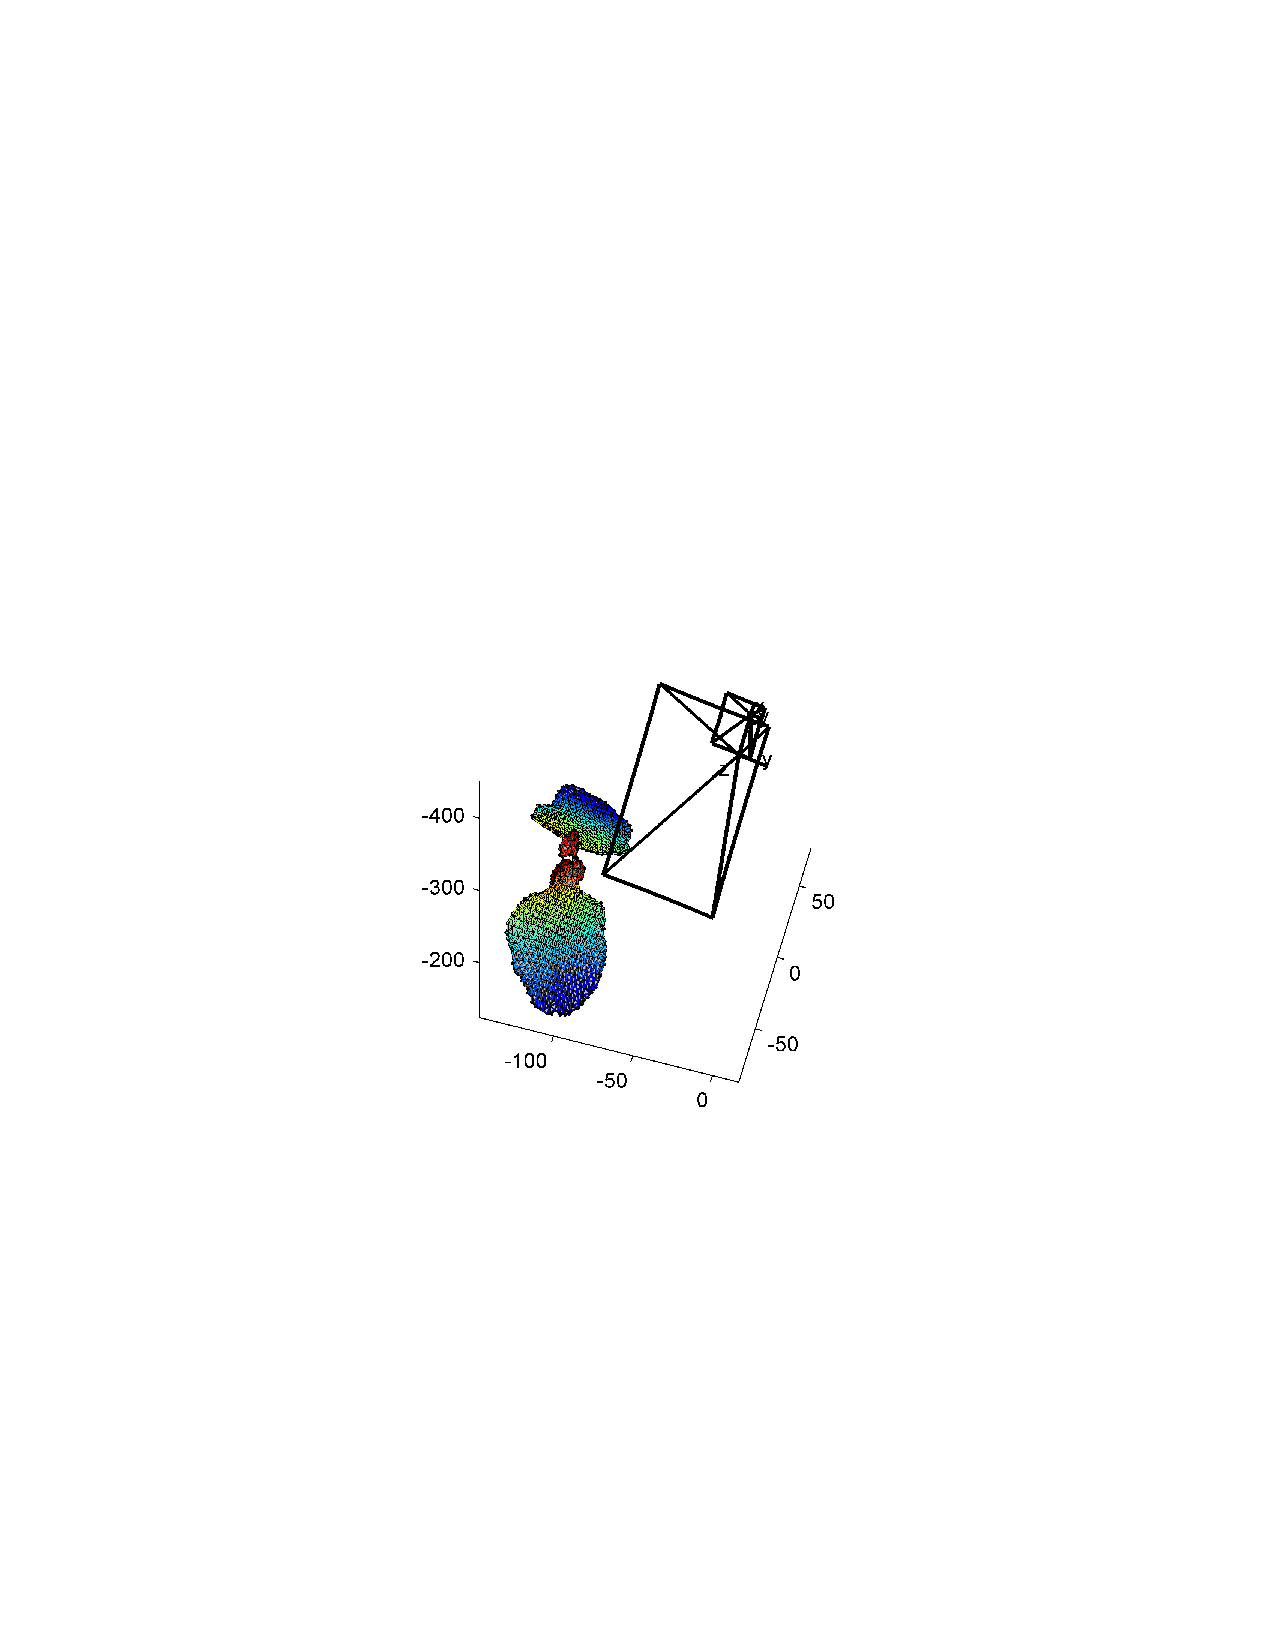
\includegraphics[trim=190 280 190 290,clip,width=0.48\linewidth]{Figures/soybean3DMeshPlusCam} &
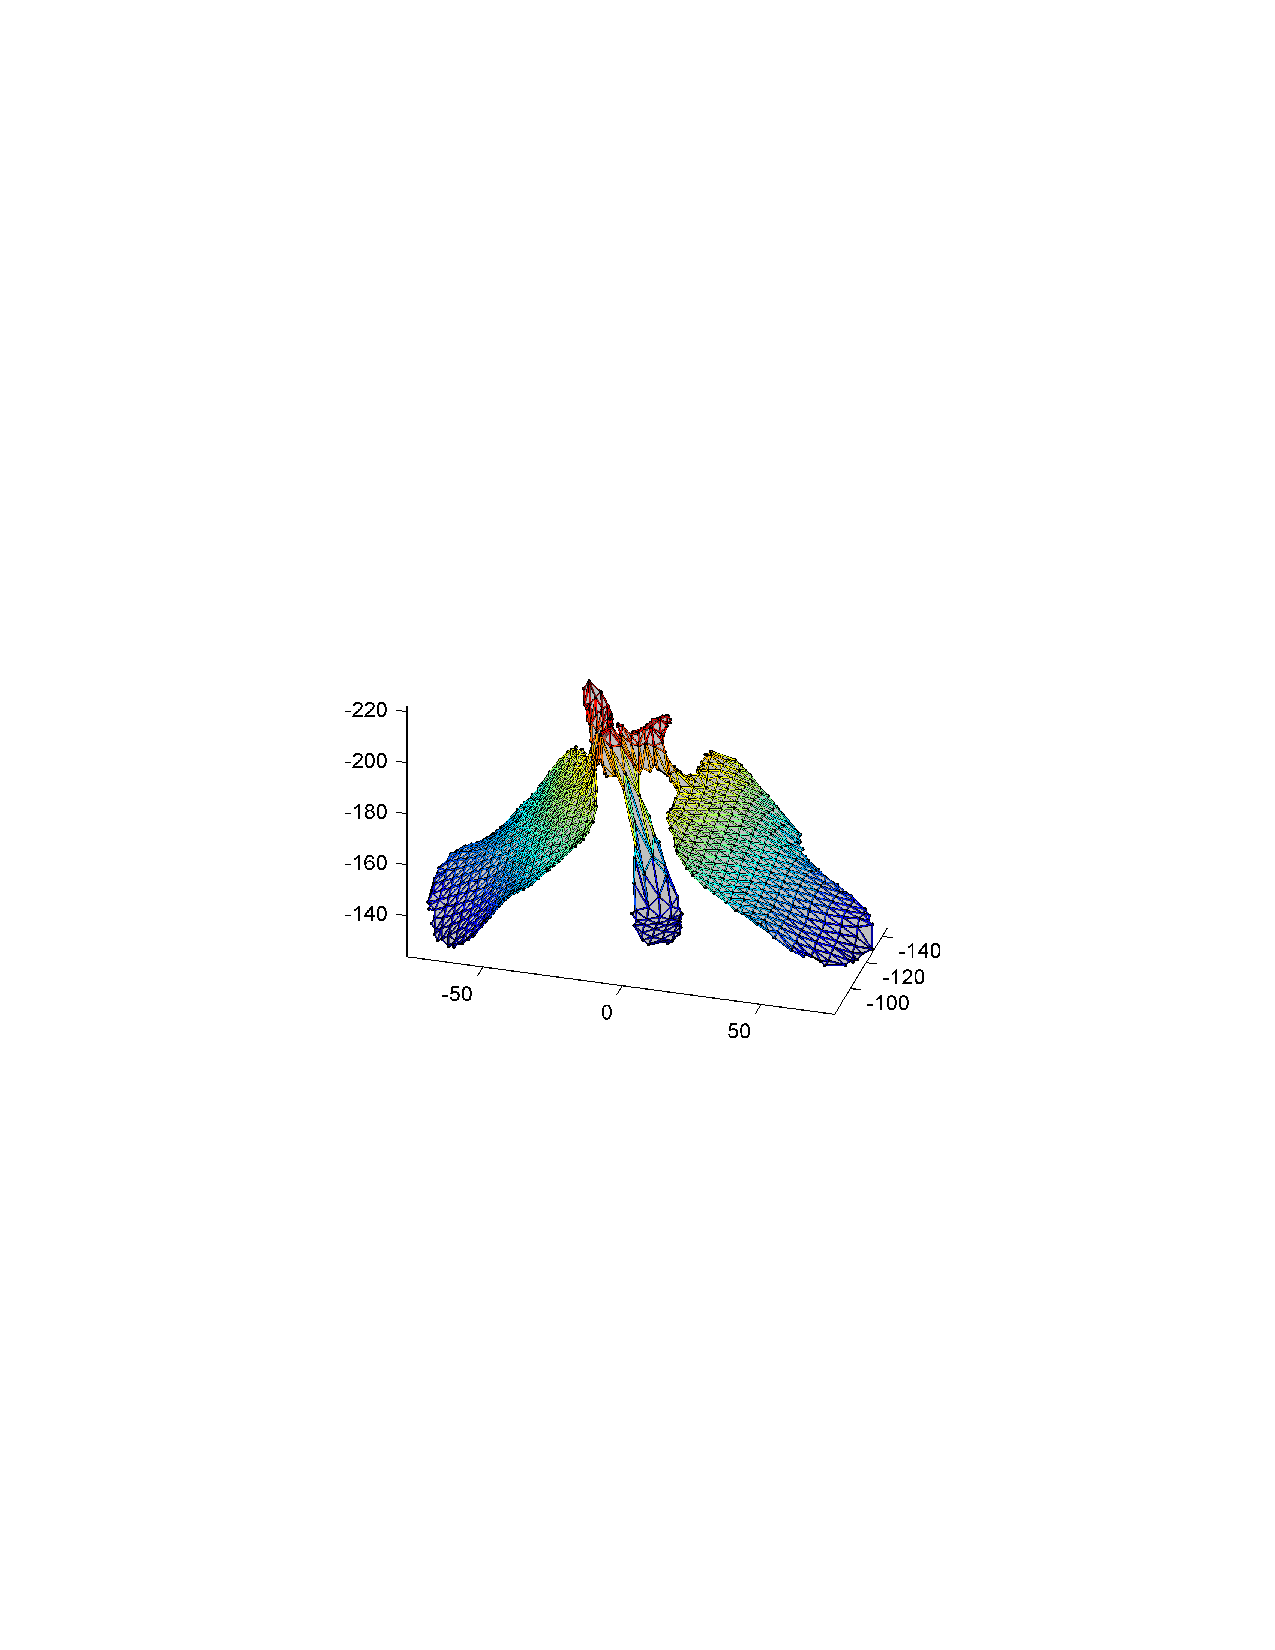
\includegraphics[trim=190 280 190 290,clip,width=0.48\linewidth]{Figures/soybean3DMesh} \\
($c$) & ($d$) \\
\end{tabular}
\end{center}
   \caption{($a$) Color image of a soybean plant.  ($b$) Mesh on the color image. ($c$) $3$D mesh along with camera poses. ($d$) Close-up of $3$D mesh.  }
\label{fig:soybean}
\end{figure}


\section{Results}
\label{sec:results}

Mesh reconstructions on a number of plants are presented.  In all 3D plots the units are millimeters.  Figure~\ref{fig:plantnoise} shows image and $3$D data, along with the estimated mesh of a potted plant.  Detailed shapes are recovered. The estimated mesh is compared to a laser scan of the same plant in Fig.~\ref{fig:plantnoiseGT}.  This shows overall good accuracy of the shape, with the main error being an extension of the leaf tip area.  It appears the lower leaf shifted in position between the laser scan and the camera image, and this may be a result of the turntable required by the laser.

Another way to quantitatively evaluate the surface is to estimate a known $3$D object.  In Fig.~\ref{fig:sphere} a 50mm diameter sphere is imaged and aligned to the points on the surface.  The $3$D point offsets from the sphere changes with the slope indicating that there are some inherent depth biases in the sensor.  Nevertheless the mesh smoothes the data noise and and approximates the sphere surface well.  The standard deviation of the raw points fit to the sphere is 2.3mm and the mesh vertices is 1.3mm.  This does not account for absolute depth error, only shape error, as the sphere center was aligned.

Surface estimates for the bean plant from Fig.~\ref{fig:beanimageprocess} are shown in Fig.~\ref{fig:beanfit}and from a soybean plant in Fig.~\ref{fig:soybean}.   The 3D points have been averaged over 30 frames to reduce noise, but still are noisy.  Despite this, mesh is able capture the leaf features well.  A comparison is made to the Marching Cube algorithm from an isosurface~\cite{Curless:1996} in Fig.~\ref{fig:beanimageprocess}($c$).  We used a modified implementation from~\cite{PVT2013} along with the Matlab isosurface command.  This shows the voxelization generating large artifacts, and using smaller voxels simply leads to surface holes.  Fig.~\ref{fig:beanfit}($d$) compares the mesh surface with a parabolic fit~\cite{Alenya2011}.  The latter gives rough shape but not a detailed model which we are able to obtain with our mesh fitting.
